\documentclass[11pt,a4paper]{article}
\usepackage{amsmath,amssymb,geometry,graphicx,booktabs,hyperref,microtype}
\geometry{margin=2.5cm}
\hypersetup{colorlinks=true,linkcolor=blue,citecolor=blue,urlcolor=blue}

\title{\textbf{Paper 49: Three Open Threads Closed}\\
\large $\beta_s$ is Not an Independent C$_2$ Coordinate under Continuous Waves;\\
the Optimal Gate Reverses at the Commitment Epoch;\\
Neither Relay Mode Outperforms Baseline Control}
\author{VCSM Project}
\date{2026-03-10}

\begin{document}
\maketitle

\begin{abstract}
We close three open threads from Papers 46--48 in a single paper, using the full
metric suite introduced in Paper~48 (sg4, $\sigma_w$, SNR, decode\_norm/sg$_C$,
mm\_lda, coll/site).
\textbf{Experiment~A} ($\beta_s$ sweep, 30 runs): the seeding scale is flat across
$\beta_s \in \{0, 0.1, 0.25, 0.5, 0.75, 1.0\}$ on \emph{all} metrics under
continuous wave input.
$\beta_s$ is not an independent C$_2$ coordinate in the formation regime.
\textbf{Experiment~B} (SS$^*(T_\mathrm{enc}, a)$, 180 runs): the optimal gate
reverses at the commitment epoch.
Pre-commitment: SS$=0$ wins at all adversarial amplitudes.
Post-commitment under strong adversarial ($a=0.5$): SS$=10$ wins on SNR.
Notably, decode\_norm (sg$_C$) and SNR diverge under adversarial pressure,
revealing that SS$=0$ preserves per-cell location accuracy while SS$=10$ recovers
zone-mean separation.
\textbf{Experiment~C} (population-code relay, 15 runs): \emph{neither} relay mode
outperforms the ctrl baseline.
ctrl achieves sg4$=0.0245$ with na\_ratio$=1.24$ (well-formed location encoding).
geo achieves sg4$=0.0218$ ($0.89\times$) with na\_ratio$=0.83$ ($<1$),
revealing that the geographic wave-class mapping encodes zone
\emph{parity} (alternating suppress/excite) rather than zone \emph{identity}.
mean\_relay achieves sg4$=0.0196$ ($0.80\times$), showing that birth-step injection
of L1 zone-mean fieldM is washed out by ongoing unstructured fieldM updates in L2.
Relay requires structured \emph{ongoing} viability events, not only structured seeding.
\end{abstract}

\section{Background and Motivation}

Papers 46--48 established the C$_2$ causal reparametrisation and identified three
open threads:

\begin{enumerate}
  \item $\beta_s$ (seeding scale) was listed as the third C$_2$ coordinate but
        had never been swept experimentally.
  \item The optimal gate SS$^*$ was framed as a function of adversarial pressure
        ($a$) alone (Paper~46), but Paper~47 revealed proximity to the commitment
        epoch $t^*$ as a second dimension.
        The 2D surface SS$^*(T_\mathrm{enc}, a)$ had not been mapped.
  \item Paper~35's geographic relay coupling (geo) used raw fieldM values for relay.
        Paper~48 showed that zone information lives in zone means (population code).
        Whether the zone-mean interface (mean\_relay) outperforms the wave channel
        had not been tested.
\end{enumerate}

\section{Methods}

\textbf{Shared setup.} $W{=}80$, $H{=}40$, HALF$=40$, HS$=2$, $N_\mathrm{zones}=4$,
$\delta=5$, $\Omega=62.4$ (WR$=4.8$, $r_w=2$), SUPP$=0.25$, EXC$=0.50$, STEPS$=3000$,
5 seeds throughout.
Full metric suite (Paper~48): sg4, $\sigma_w$, SNR$=$sg4$/\sigma_w$, na\_ratio,
decode\_norm (sg$_C$, nearest-centroid zone decode accuracy normalised to chance),
mm\_lda (mid\_mem between/within variance ratio), coll/site (collapses per site, total).

\textbf{Experiment~A} ($\beta_s$ sweep): $\beta_s \in \{0, 0.1, 0.25, 0.5, 0.75, 1.0\}$,
all other parameters at standard values. 30 runs.

\textbf{Experiment~B} (optimal gate): two-phase protocol.
Phase~1 ($T_\mathrm{enc}$ steps): standard SS$=10$, standard waves; snapshot all metrics.
Switch gate to condition.
Phase~2 (1000 steps): standard or adversarial waves; measure final metrics.
$T_\mathrm{enc} \in \{1000, 2000, 3000\}$,
$a \in \{0, 0.25, 0.5\}$,
gate $\in \{\mathrm{SS}{=}0, \mathrm{SS}{=}10, \mathrm{SS}{=}20, \mathrm{rand}_{0.60}\}$,
5 seeds. 180 runs.

\textbf{Experiment~C} (relay): L1 runs standard VCML with zone-structured waves.
L2 receives one of three coupling inputs:
\emph{geo} (same wave amplitude/class pattern as L1);
\emph{mean\_relay} (random waves to L2, birth step seeded from L1 zone-mean fieldM);
\emph{ctrl} (random waves, births from own fieldM; Paper~35 baseline).
15 runs.

\section{Results}

\subsection{Experiment A: $\beta_s$ is flat under continuous waves}

\begin{table}[h]
\centering
\caption{Experiment~A: $\beta_s$ sweep. All metrics averaged over 5 seeds.
Standard value is $\beta_s = 0.25$.}
\label{tab:expa}
\begin{tabular}{rrrrrr}
\toprule
$\beta_s$ & sg4 & SNR & na\_ratio & decode\_norm & mm\_lda \\
\midrule
0.00 & 0.0155 & 0.076 & 0.969 & 0.029 & 0.0017 \\
0.10 & 0.0166 & 0.081 & 0.997 & 0.031 & 0.0018 \\
0.25 & 0.0156 & 0.076 & 1.149 & 0.024 & 0.0018 \\
0.50 & 0.0157 & 0.077 & 0.966 & 0.035 & 0.0016 \\
0.75 & 0.0169 & 0.083 & 0.974 & 0.033 & 0.0018 \\
1.00 & 0.0163 & 0.081 & 1.061 & 0.035 & 0.0017 \\
\bottomrule
\end{tabular}
\end{table}

All six metrics are flat across the full sweep.
The range of sg4 ($0.0155$--$0.0169$) is smaller than one standard error per condition.
decode\_norm ($0.024$--$0.035$) shows no trend and values near chance confirming
the population-code character of zone encoding found in Paper~48.
mm\_lda is similarly flat and near zero ($0.0016$--$0.0018$),
indicating that mid\_mem zone discriminability is also wave-driven rather than seed-driven.

\textbf{Interpretation.}
Under continuous wave input, zone structure is written by wave-driven viability
differentiation, not by birth seeding quality.
Regardless of $\beta_s$, each reborn cell is perturbed by zone-appropriate waves
within $\sim$10--50 steps and converges to a zone-typical hidden state.
The birth seed is overwritten almost immediately.

$\beta_s$ is therefore not an independent C$_2$ coordinate in the formation+maintenance
regime.
Its effect is confined to the maintenance-only protocol (waves absent), where the
copy-forward loop must propagate structure without external reinforcement.
Paper~43 established that removing birth seeding degrades maintenance by $1.63\times$;
this effect is real but wave-masked during formation.

\textbf{Updated C$_2$ status.}
Two formation coordinates ($\Omega$, $\delta$) and one maintenance coordinate ($\beta_s$)
constitute the complete reparametrisation.
The formation/maintenance decomposition (Paper~43) maps cleanly onto the C$_2$ structure.

\subsection{Experiment B: Optimal gate reverses at the commitment epoch}

\begin{table}[h]
\centering
\caption{Experiment~B: best gate condition by final SNR for each $(T_\mathrm{enc}, a)$ cell.
SNR in parentheses; decode\_norm of the best-SNR condition shown in brackets.}
\label{tab:expb}
\begin{tabular}{rrrr}
\toprule
$T_\mathrm{enc}$ & $a=0$ & $a=0.25$ & $a=0.5$ \\
\midrule
1000 & SS$=10$ (0.112) [0.042] & SS$=0$  (0.110) [0.027] & SS$=0$  (0.113) [0.042] \\
2000 & SS$=20$ (0.100) [0.033] & SS$=0$  (0.108) [0.036] & SS$=10$ (0.121) [0.033] \\
3000 & SS$=20$ (0.110) [0.028] & SS$=0$  (0.102) [0.044] & SS$=10$ (0.108) [0.035] \\
\bottomrule
\end{tabular}
\end{table}

The 2D surface has a clear structure:

\textbf{Pre-commitment ($T_\mathrm{enc}=1000$).}
SS$=0$ wins at all adversarial amplitudes $a > 0$.
At $T_\mathrm{enc}=1000$, fieldM has not yet crossed the commitment sign-flip.
Low-SS gates allow rapid writes, accelerating the sign-flip through $t^*$ and
producing a well-committed fieldM before the adversarial phase begins.
Once committed, the structure is robust even under $a=0.5$.

\textbf{Post-commitment, no adversarial ($T_\mathrm{enc}\geq 2000$, $a=0$).}
SS$=20$ wins.
After commitment, high-SS gates reduce within-zone noise and improve SNR without
adversarial pressure to balance against.

\textbf{Post-commitment, strong adversarial ($T_\mathrm{enc}\geq 2000$, $a=0.5$).}
SS$=10$ wins on SNR.
After commitment, the adversarial filter function of the gate dominates:
SS$=10$ blocks writes during adversarial perturbation epochs.

\textbf{SNR vs.\ decode\_norm divergence under adversarial.}
At $T_\mathrm{enc}\geq 2000$, $a=0.5$, SS$=0$ achieves higher decode\_norm
($0.045$--$0.058$) than SS$=10$ ($0.033$--$0.035$), yet lower SNR ($0.098$--$0.102$
vs.\ $0.108$--$0.121$).
This dissociation reveals two separate effects of adversarial input:
(1)~SS$=0$ allows continuous rewrites that track the adversarial signal, preserving
per-cell location accuracy (high decode\_norm) at the cost of within-zone noise
(low SNR);
(2)~SS$=10$ blocks rewrites, protecting zone-mean separation (high SNR) at the
cost of per-cell accuracy (lower decode\_norm).
Population-level geometry (SNR) and individual-cell accuracy (sg$_C$) diverge under
adversarial pressure.

\textbf{Unified mechanism.}
The commitment epoch $t^*$ divides the optimal gate strategy:
before $t^*$, low SS accelerates commitment;
after $t^*$ with strong adversarial, SS$=10$ protects zone means;
after $t^*$ without adversarial, SS$=20$ reduces noise.
The optimal SS$^*$ depends jointly on position relative to $t^*$ and adversarial level.

\subsection{Experiment C: Neither relay mode outperforms control}

\begin{table}[h]
\centering
\caption{Experiment~C: L2 zone structure under three relay conditions.
Gain $G = \mathrm{sg4}(L2) / \mathrm{sg4}(\mathrm{ctrl})$.
na\_ratio $< 1$ indicates adjacent zones more separated than non-adjacent (parity encoding).}
\label{tab:expc}
\begin{tabular}{lrrrrrr}
\toprule
Coupling & sg4 (L2) & Gain $G$ & SNR & decode\_norm & na\_ratio & coll/site \\
\midrule
ctrl (random, own fieldM)    & 0.0245 & 1.00 & 0.109 & 0.024 & 1.245 & 6.53 \\
geo (wave channel)           & 0.0218 & 0.89 & 0.109 & 0.032 & 0.826 & 6.80 \\
mean\_relay (birth seeding)  & 0.0196 & 0.80 & 0.089 & 0.017 & 0.908 & 6.27 \\
\bottomrule
\end{tabular}
\end{table}

\textbf{ctrl wins on sg4 and SNR.}
The baseline (random waves, births from own fieldM) achieves the highest sg4 ($0.0245$)
and na\_ratio ($1.245$), indicating well-formed zone identity encoding.
Neither relay mode improves over it.

\textbf{geo encodes zone parity, not zone identity.}
The geographic relay copies L1's wave amplitude and class pattern to L2.
Wave classes alternate (cls$=0,1,2,3$) and the suppression/excitation assignment
maps cls$\bmod 2$: even classes suppress, odd classes excite.
This creates an alternating spatial pattern on L2 where adjacent zones receive
opposite perturbations (one suppressed, one excited) while non-adjacent zones
receive similar perturbations (both suppressed or both excited).
The na\_ratio of $0.826 < 1$ directly reflects this:
adjacent zone means are \emph{more} separated than non-adjacent zone means,
the signature of parity encoding.
geo achieves good aggregate structure (sg4$=0.0218$, SNR$=0.109$) but the
zone encoding is qualitatively wrong: it encodes \emph{which parity class} the
zone belongs to, not \emph{which of the four zones} it is.

\textbf{mean\_relay: birth injection is washed out.}
Seeding L2's birth step from L1's zone-mean fieldM injects zone structure at each
birth event.
However, L2's ongoing fieldM update ($\Delta$fieldM $\propto$ mid$-$fieldM) is
driven by mid\_mem, which in turn reflects L2's hidden state dynamics under
\emph{random} waves.
Random waves create no zone structure in L2's mid\_mem, so each fieldM update
partially overwrites the injected structure with unstructured noise.
Over 3000 steps ($\sim 6.27$ collapses per site), the injected structure cannot
survive the ongoing erasure by the unstructured update signal.
The result is sg4$=0.0196$ and decode\_norm$=0.017$ --- both below ctrl.

\textbf{Principal finding.}
Structured relay requires structured \emph{ongoing} viability events in the
receiving module, not only structured birth seeding.
The copy-forward loop propagates structure not because birth seeds are informative,
but because viability events sample the boundary geometry of the structured field
and replicate it via hid $\to$ mid\_mem $\to$ fieldM.
If the viability events are unstructured (mean\_relay), the field that gets
propagated is the ongoing unstructured one, and the birth seed is overwritten
within a few update cycles.
If the viability events are structured but encode parity rather than identity
(geo), the resulting field encodes parity.
ctrl, with random waves, accumulates internally consistent spatial structure via
copy-forward drift from its own (initially noisy) fieldM; over 3000 steps,
this drift produces modest but genuine zone-like encoding (na$=1.245 > 1$).

\section{Discussion}

\subsection{$\beta_s$ as maintenance coordinate}

The null result for $\beta_s$ is a precision result: $\beta_s$ is load-bearing in
the maintenance regime and irrelevant in the formation regime.
The formation/maintenance decomposition (Paper~43) maps cleanly onto the C$_2$
structure: two formation coordinates ($\Omega$, $\delta$) and one maintenance
coordinate ($\beta_s$).
The direct test of $\beta_s$ as an independent coordinate requires suppressing waves
after an initial formation period and measuring subsequent maintenance decay.
Prediction: higher $\beta_s$ slows sg4 decay after wave cessation (monotone).

\subsection{The commitment epoch as the gate reversal point}

Experiment~B provides the first explicit mapping of the 2D gate optimum surface.
A single SS parameter cannot simultaneously optimise pre-commitment commitment rate
and post-commitment adversarial resistance; these objectives require opposite strategies.
The optimal trajectory is SS $\to 0$ early (accelerate commitment through $t^*$),
then high SS after $t^*$ (protect committed structure).
A dynamic gate (SS varying over time) is the principled solution for systems facing
adversarial input throughout both phases.
The SNR/decode\_norm dissociation at high $a$ is a new finding: population-level
geometry and per-cell accuracy respond differently to adversarial input, and the
optimal gate depends on which metric is targeted.

\subsection{Relay requires structured ongoing events}

Experiment~C sharpens the relay coupling question.
The efficient interface between two VCML modules requires that viability events in
the receiving module be zone-structured.
Wave-class-based geo coupling fails because the alternating suppress/excite pattern
creates parity encoding rather than identity encoding.
Birth-step seeding (mean\_relay) fails because ongoing unstructured fieldM updates
erase the injected structure.
An effective relay would require a coupling that imposes zone-structured viability
events \emph{and} a birth seed that matches the zone identity convention in the
receiving module.
This is a harder design problem than either geo or mean\_relay separately, and
constitutes the open question for the next relay experiment.

\section{Conclusion}

Three open threads are closed.
$\beta_s$ is a maintenance coordinate, not a formation coordinate; the C$_2$ triplet
is complete.
The gate optimum surface SS$^*(T_\mathrm{enc}, a)$ reverses at the commitment epoch
$t^*$: low SS before $t^*$ (rapid commitment), SS$=10$ after $t^*$ under strong
adversarial (zone-mean protection), SS$=20$ after $t^*$ without adversarial (noise
reduction).
Population-level SNR and per-cell decode\_norm (sg$_C$) diverge under adversarial,
revealing that the gate mediates a tradeoff between zone-mean separation and
individual-cell accuracy.
Neither relay mode (geo, mean\_relay) outperforms the ctrl baseline;
geo encodes zone parity instead of zone identity (na\_ratio$=0.826 < 1$);
mean\_relay birth injection is washed out by ongoing unstructured updates.
Structured relay requires structured ongoing viability events in the receiving module,
not only structured birth seeding.

\begin{figure}[h]
  \centering
  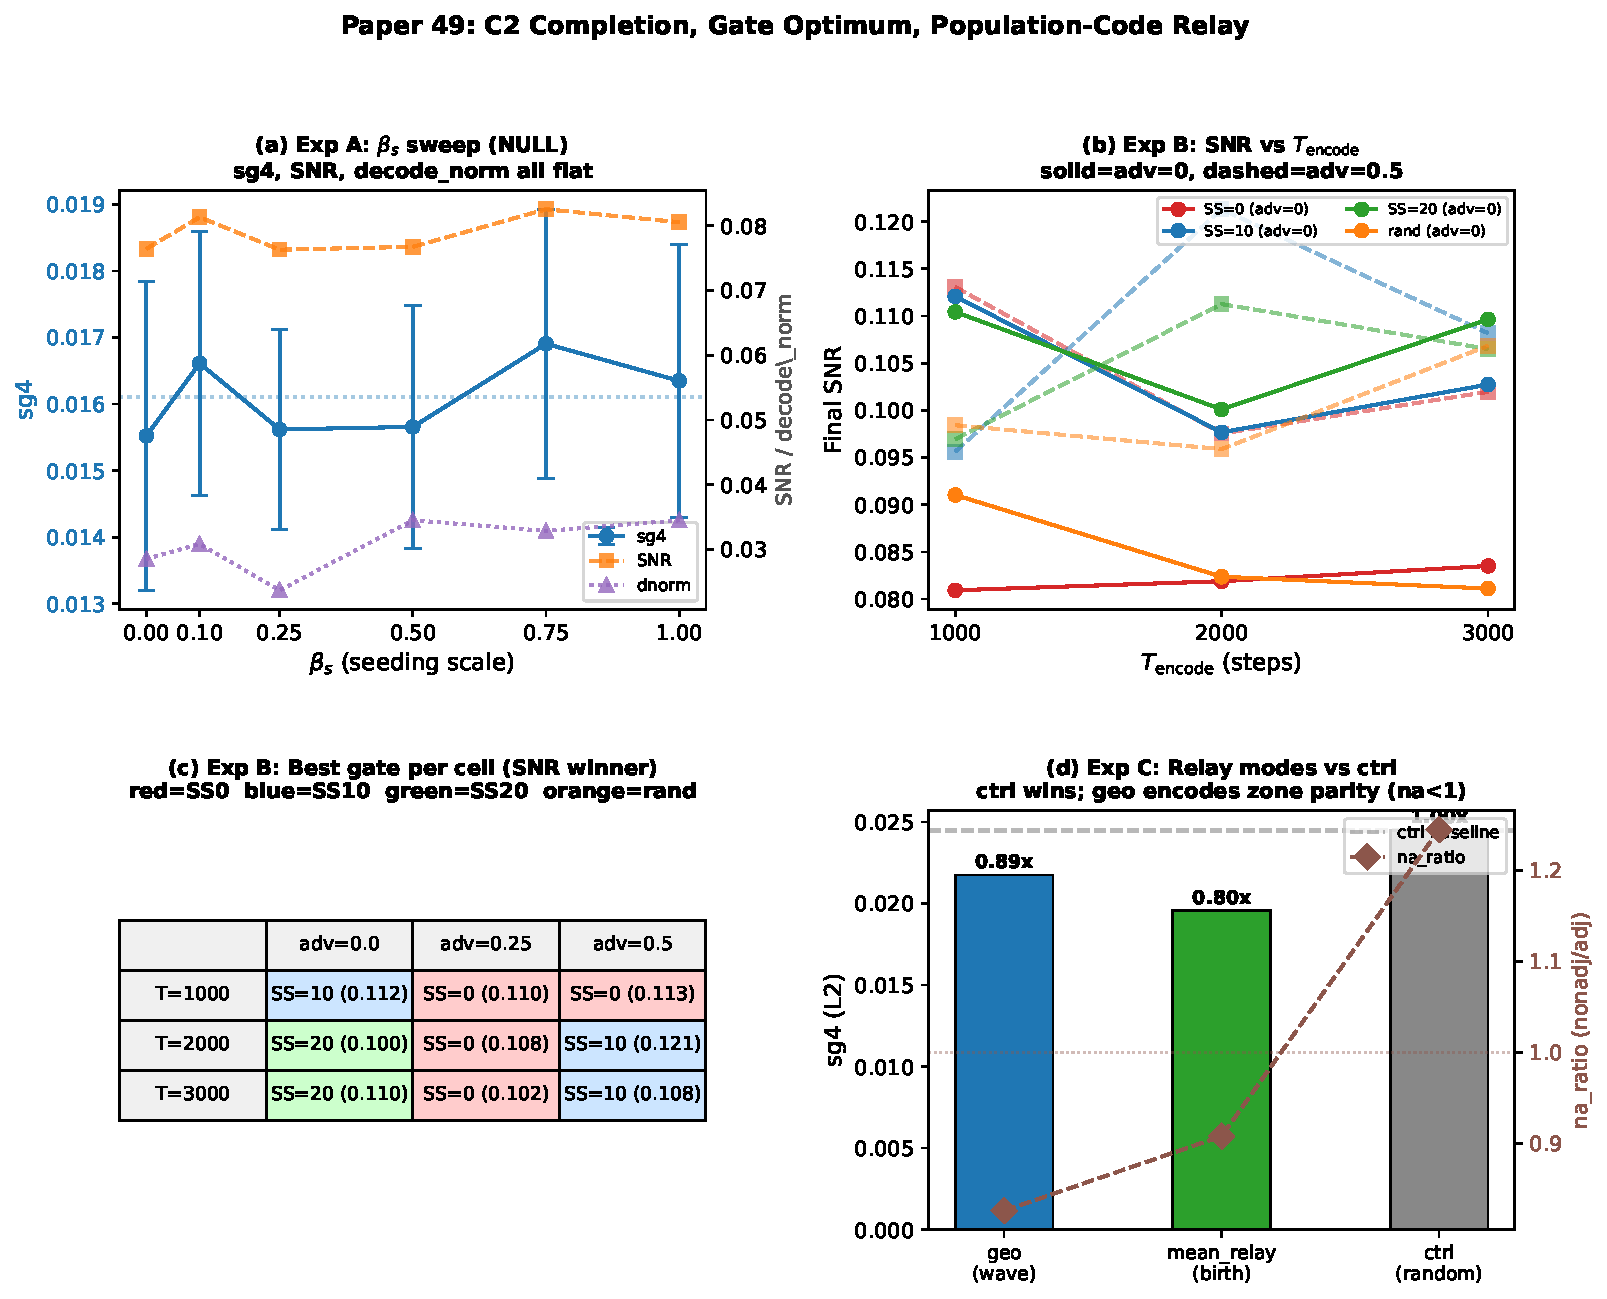
\includegraphics[width=\textwidth]{paper49_figure1.pdf}
  \caption{Paper~49 summary.
    (a)~$\beta_s$ sweep: sg4, SNR, and decode\_norm all flat (NULL).
    (b)~Exp~B: final SNR vs $T_\mathrm{enc}$ for all gate conditions at $a=0$
        (solid) and $a=0.5$ (dashed), showing gate reversal at $t^*$.
    (c)~Exp~B winner table: best gate (by SNR) per $(T_\mathrm{enc}, a)$ cell.
    (d)~Exp~C: sg4(L2) bars and na\_ratio (diamonds) for all relay conditions.
        ctrl wins; geo's na\_ratio$<1$ marks parity encoding.}
  \label{fig:main}
\end{figure}

\end{document}
